\subsection{Image Processing}
In the previous sections we have learned about two different approaches to train neural nets on solving certain tasks. Although we came to understand that the complexity of the task to be solved correlates strongly with the amount of data at hand, there exist domains from which it is undeniably easier to do so. To equip a neural net with some sort of prior knowledge by switching the domain may therefore not only be highly desirable but sometimes also needed if the amount or quality of data is not sufficient. One domain which is of special interest when it comes to interacting in a three dimensional environment is a domain that represents depth information. If there are any, it may sometimes be possible to extract this kind of prior knowledge from a depth camera. As for this work, we need to rely on stereo cameras and powerful algorithms that allow us to compute depth images in real time. The algorithm that helps us to do so, in terms of the extraction of weighted least squares disparity maps, will be presented in the following paragraph - Depth Map Extraction.
\subsubsection{Depth Map Extraction}
As already pointed out, the depth map is generated from stereo camera images by a technique called stereo matching \cite{hamzah2010sum}. This method works best for  
\begin{figure}[h]
	\centering
	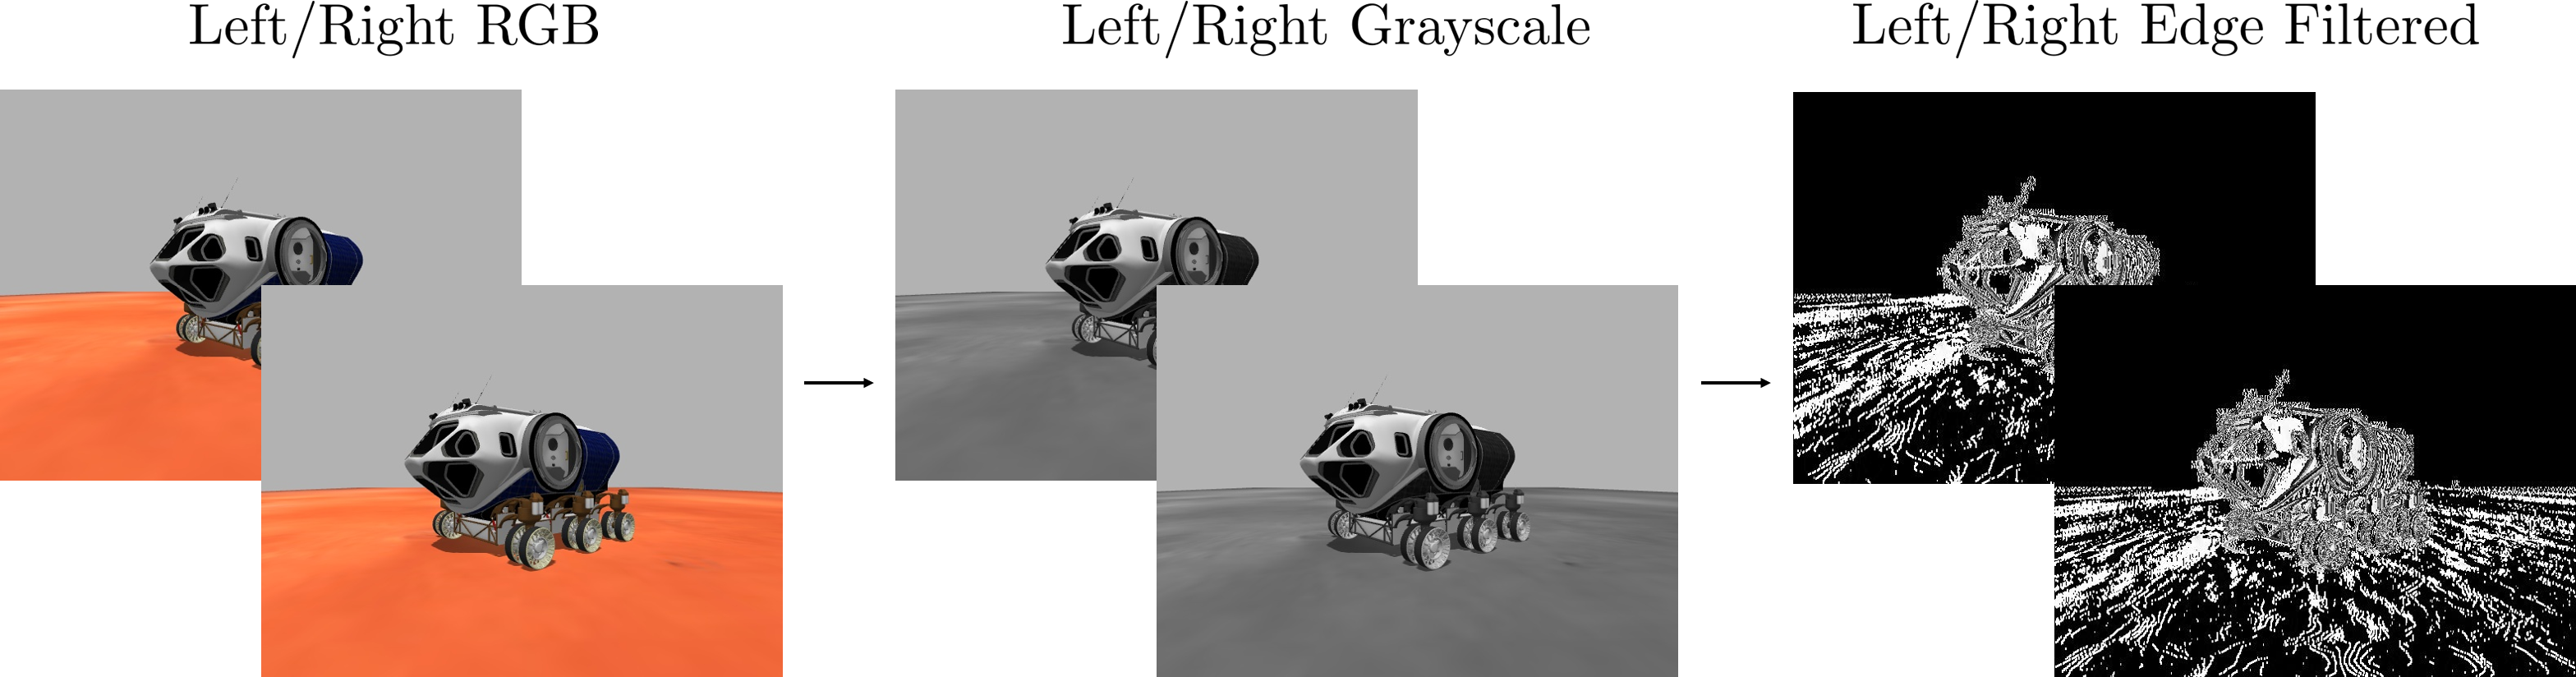
\includegraphics[scale=.25]{chapters/03_background/img/image_preprocessing.png}
	\caption{}
	\label{fig::323_image_preprocessing}
\end{figure}
\begin{figure}[h]
	\centering
	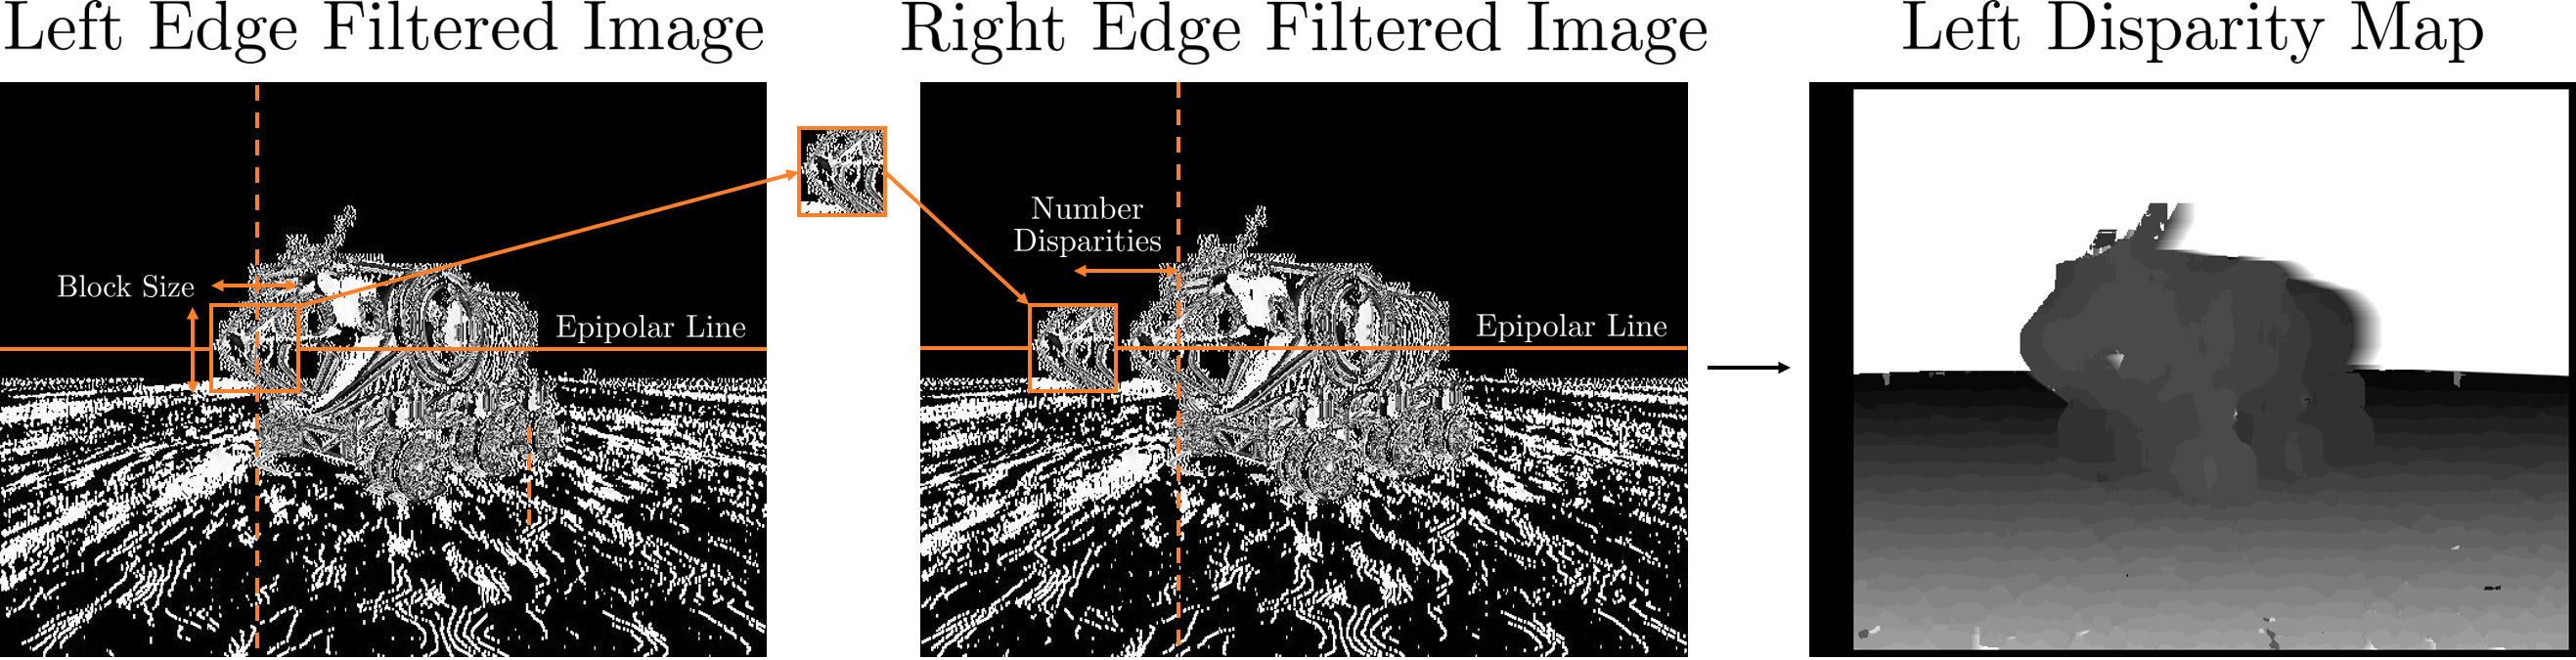
\includegraphics[scale=.3]{chapters/03_background/img/left_disparity_map.png}
	\caption{}
	\label{fig::323_left_disparity_map}
\end{figure}
\cite{sobel2014an}   sobel\\
\cite{hamzah2010sum} stereo matching\\
\cite{egnal2004stereo} left right consistency\\
\cite{min2014fast}   wls\\
\cite{tomasi1998bilateral} bilateral
\\\\
As a requirement for the algorithm to work properly, it is important to calibrate the robot's cameras. Therefore, the next chapter - Mono and Stereo Camera Calibration, will explain in detail why, and how to calibrate cameras.
\subsubsection{Mono and Stereo Camera Calibration}